\documentclass[a4paper,landscape]{article}
\usepackage{xcolor}
\usepackage{fullpage}
\usepackage{graphicx}
\usepackage{epstopdf}
\usepackage{caption}
\usepackage{verbatim}
\usepackage{amssymb}
\usepackage{amsmath,amsthm}
\usepackage{amsfonts}
\usepackage{enumerate}
\usepackage{enumitem}
\usepackage{listings}
\usepackage{qtree}
\usepackage{tikz}
\usepackage{bm}
\usepackage{lscape}
\usepackage{frame,color}
\usepackage{datetime}
\usepackage{etoolbox}
\usepackage{emerald}
\usepackage{multicol}
\usepackage[T1]{fontenc}
\title{<Title Goes Here>}
\date{}
\author{}
\makeatletter
\patchcmd{\chapter}{\if@openright\cleardoublepage\else\clearpage\fi}{}{}{}
\makeatother
\definecolor{shadecolor}{rgb}{184,184,184}
\lstset{language=Matlab,
        frame = single,
        breaklines=true
}
\usetikzlibrary{calc,positioning}
\usetikzlibrary{arrows,automata}
\renewcommand{\familydefault}{\sfdefault}
\setlength{\columnsep}{2cm}
\begin{document}
%\begin{landscape}

%%%%%%%%%%%%%%%%%%%%%%%%%%%%%%%%TITLE PAGE%%%%%%%%%%%%%%%%%%%%%%%%%%%%%%%%%%%%%%%%%%%%%%%%

\begin{figure}
    \begin{minipage}[H]{0.33\textwidth}
    \begin{flushleft}
   		\vspace{0.3cm}
		
\includegraphics[scale=0.8]{images/TUDelftLogo.eps}
	\end{flushleft}
	\end{minipage}
	\begin{minipage}[H]{0.33\textwidth}
		\begin{center}
			\ECFJD{Context Project Group 8}
		\end{center}
		
		\begin{center}
			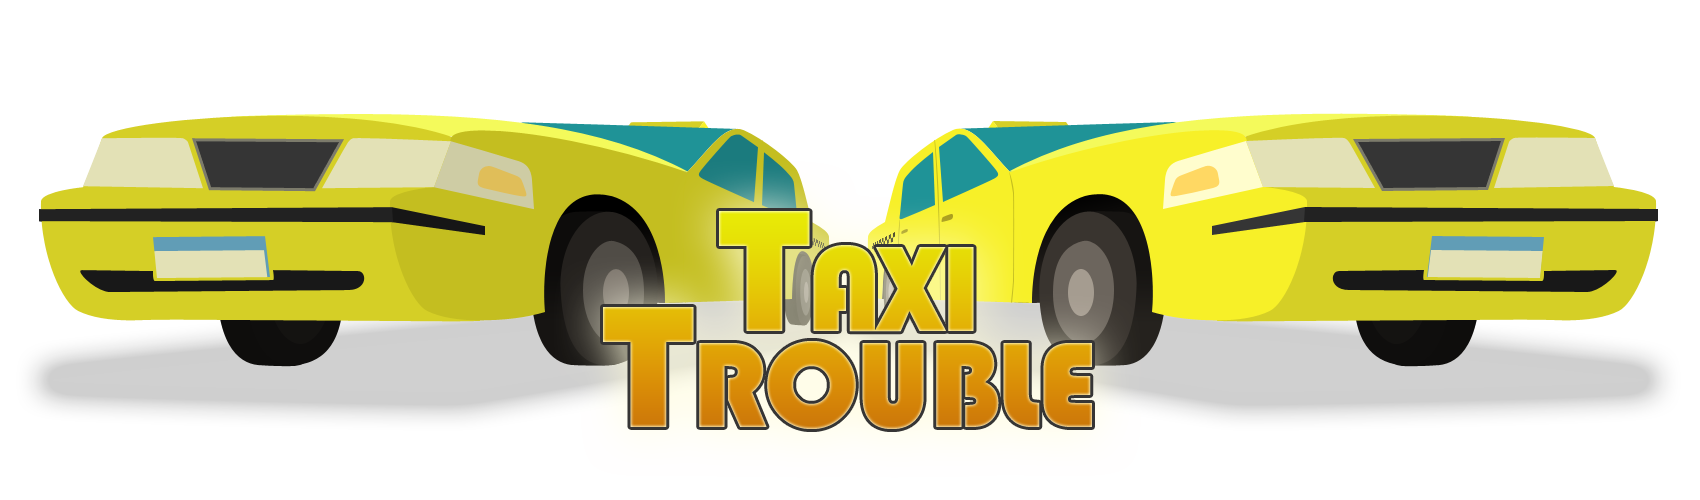
\includegraphics[height=2cm]{images/tt.png}	
		\end{center}
	 	\end{minipage}
	\begin{minipage}[H]{0.33\textwidth}
			\begin{flushright}
				\small{Rob van Bekkum \qquad rvanbekkum\qquad 4210816}\\
				\small{Thijs Brands \qquad tlmbrands\qquad 4247132}\\
				\small{Soheil Jahanshahi \qquad sjahanshahi\qquad 4127617}\\
				\small{Aidan Mauricio \qquad amauricio\qquad 4195175}\\
				\small{Joost van Oorschot\qquad jjevanoorschot\qquad  4220471}\\
				\vspace{0.2cm}
			\end{flushright}
			
	\end{minipage}
	\end{figure}
%%%%%%%%%%%%%%%%%%%%%%%%header ends here%%%%%%%%%%%%%%%%%%%%%%%%%%%%%%%%%%%%%%%%%%%%%%%%
\maketitle	
	\section{Introduction}
	This document has been written with the goal of providing insight in the architecture design of our software solution. The architecture design will be subjected to change frequently due to the need for additional features or problems encountered with the current design. This document will be updated accordingly when these changes are made.
	\section{Overview}
	What we would like to include in this section is:
\begin{enumerate}
	\item Brief description of the game (not elaborate as in the product vision)
	\item Give an overview of all of the functionalities that are included and implemented
	in the final version of the game:
	\begin{enumerate}
		\item \textbf{Driver and navigator screens of the game.} Tell something about the roles and
		different views corresponding to those roles in the game.
		\item \textbf{Teams of drivers and navigators}: Description of in which way teams are formed,
		i.e. each team consists of a driver and navigator.
		\item \textbf{Taxis}: Controllable by a driver and collidable with other taxis.
		\item \textbf{Passengers}: pickup, drop-off and stealing
		\item \textbf{Power-ups}: can be picked up by the driver and activated by navigator, there are different types
		\item \textbf{Game Head Up Display}: displays team, score and time left in the game
		\item \textbf{Sound effects}: different sound effects for different events
		\item \textbf{Menu Screen}: when the game starts, you can either start the game or check out the leaderboard
		\item \textbf{Multiplayer implementation}: invitations via Google account, player can set the preferred number of
		      other players, team score is submitted on the leaderboard when the game ends.
	\end{enumerate}
\end{enumerate}
	\section{Functionalities}
	\begin{itemize}
	\item Driver and Navigator Screen
	\begin{item}
		\item \textbf{Driver screen} has myopic 2d view of the map where it makes driver's sight limited such that it is impossible to win the game without cooperation.There are touchscreen controls that is used by driver to control the taxi's acceleration and direction.   
		\item \textbf{Navigator Screen} has the 2d zoom-able screen in top view and Navigator gets the whole map overview. There is a power-up button where is controlled by Navigator and can be activated at the right moment by him/her.
	\end{item}
	\item Teams 
	\begin{item}
		\item  Teams is made of two participants where each will takes a role in the game; Either as an driver or Navigator. After all the required teams(from 2-4 teams) are created the game begins.
	\end{item}	
	\item Taxi
	\begin{item}
		\item Taxi is a solid object , it has wheels that controls steering and acceleration which is controlled by driver.
		\item When two taxis collide with each other, collision is detected and natural reflection of the taxi body upon collision is performed.  
	\end{item}	
	\item Passenger
	\begin{item}
		\item Passenger is an entity where are spawned in random locations in the map.
		\item There are different looks of a passenger(girl, boy, man) 
		\item each passenger is spawned in random location ready to be picked up by taxi.
		\item passengers can be stolen by other taxi while on their way to destination.
		\item Destination is assigned to each passenger which is dropped off by taxi in the game.
		\item when passenger is picked up by taxi, drop off timer is started and in order to achieve score taxi need to drop passenger off before drop off timer ends.
	\end{item}	
	\item Power-ups
	\begin{item}
		\item There are three types of power-ups(invincibility, speed boost, increase drop off timer)
		\item Invincibility power up is made when taxi wants to protect the passenger from getting stolen.
		\item Speed boost when activated will increase the acceleration of taxi from  10 second
		\item Increase drop off powerup will extra 10 second to the time that needs to be dropped off by passenger   
	\end{item}	
	\item Game Head Up Display
	\begin{item}
		\item displays team : textual representation of team numbers 
		\item score : achieved score 
		\item time left in the game : count down timer indication time left for taxi to drop passenger at his/her destination
	\end{item}	
	\item Sound effects
	\begin{item}
		\item Sound effect is activated at the time when events such as taxi collision, passenger pickup/drop off/stealing happens. 
	\end{item}	
	\item Menu Screen
	\begin{item}
		\item Play button: when play button is pushed the player is guided to the room, from there player either can find random people or invite their friends from Google+ to team up with friends. 
		\item Leaderboard: player can view the top scores of all participants so far, friend’s scores is shown highlighted.
	\end{item}	
	\item Multiplayer
	\begin{item}
		\item Multiplayer is formed via invitation of other participants 
		\item player can set the preferred number of other players to play with the boudary is from 2 to 4 teams 
		\item team score is submitted on the leader-board when the game ends.
		\item all teams are concurrently updated on the events that are happening inside the game environment.
	\end{item}	
\end{itemize}
	\section{Interaction Design}
	After seven weeks of development we conducted a user test among visitors of the TU Delft Science Center. This section will describe the Interaction Design aspects of the usability evaluation that we conducted there. Firstly, we will discuss our evaluation methods and what part of the system we tested. Secondly, we will give an overview of how the testing was done, by discussing the setting and location of the user test, a description of the users that tested the game, and the methods that we used during the test. Lastly, we will give a summary of our findings.
\\\\
For the usability evaluation, we have chosen to use the empirical 'experiment' practice. An experiment was best suited for our user test, because we wanted to observe users interact with the game in order to discover flaws in the game, and to identify gameplay elements that were not considered fun. A big aspect of Taxi Trouble is communication, which resulted in users practicing Think Aloud without being asked by us. This was very useful for our evaluation of the user test, as it gave us a lot of information about how the users perceived the game.

The usability evaluation was done right before the release of the beta release of Taxi Trouble, so that we could incorporate our findings into the beta version. This means that we evaluated the usability of the alpha version of Taxi Trouble. The alpha version was missing a lot of features compared to the final version, but it was stable enough to conduct a user test with.
\\\\
For the setting of the user test we chose the TU Delft Science Center. The Science Center is a good location for testing because it receives a lot of visitors that fit into the user demographic of Taxi Trouble, and there are sufficient facilities for conducting a user test. We were appointed a large, open room, with two racing chairs in the center of the room. The racing chairs made the user test more fun for the younger users, and fit the theme of Taxi Trouble well.

The users that tested Taxi Trouble ranged in age from $8$ to $24$. We took great care during the user tests with the younger users. The parents of the younger users were present during the user tests at all times and we made sure to mention that the users could stop the test at any time.
\\\\
The user test was performed in groups of two users. At the start of the test we asked the users to sit next to each-other and to pick a role in the game (either navigator or driver). Then, we let the users play the game for about five minutes. During this time we logged what the users said to each-other and we did not interact with the users. After playing the game, we interviewed the users about the game, asking open questions about the art style of the game, the controllability of the game, and about the gameplay.
\\\\
We did a formative evaluation of the test resuslts and we will give a summary of our findings in this section. Overall, the users were very pleased with our game. Even though all users stated that they found the controllability of the game sufficient, we noticed that most users struggled to understand what the buttons to control the car meant, and they had to take some time to figure that out by trial-and-error. This resulted in us creating buttons that mimicked the look of an actual gas pedal and brake.

During the evaluation it became apparent that users did not immediately understand the navigator view. To make the navigator screen more understandable, we created a HUD that shows to which team the navigator belongs.

Another thing that we found out, is that when a taxi is carrying a passenger, it is hard for the users to distinguish the front of the taxi from the back. In response to this we created new sprites for the taxi that clearly show the difference between the front and back of the car.

The results of the usability evaluation helped us identify a number of flaws, which allowed us to fix them. Additionally, we were able to pinpoint which gameplay features the users liked and which features they disliked.
	\section{Evaluation of Functional Modules}
	What we would like to include in this section is:
\begin{enumerate}
	\item Table with overall evaluation results from user tests.
	\item Evaluation of individual functional modules (with more specific feedback we got from the users):
	\begin{enumerate}
		\item \textbf{Driver controls} 
		\item \textbf{Navigator controls}
		\item \textbf{Picking up and dropping of passengers}
		\item \textbf{Stealing passengers}
		\item \textbf{Power-ups}
		\item \textbf{Game Head Up Display}
		\item \textbf{Sound effects}
		\item \textbf{Menu Screen}
		\item \textbf{Multiplayer implementation}
	\end{enumerate}
\end{enumerate}
	\section{Outlook}
	After delivering a product that satisfies our expectations and our end user's needs there is always room for improvement. Taxi Trouble is playable and lots of fun to play, but it still contains a few bugs. Also there are tons of features that didn't make the first release of the game which could still be implemented in the future. Implementing these will greatly increase the quality and the experience of the user who plays the game.\\

\subsection*{Bugs}
A bug is a flaw in the software. The two bugs that are present in Taxi Trouble are namely:
\begin{itemize}
\item When the Host of the game locks his phone or minimizes the game all messages stop getting through meaning that the features of the game won't work until the host resumes the game again.
\item If you want to restart the game to play again you need to completely kill the app or the game will not start correctly anymore.
\end{itemize} 
Solving these bugs will greatly increase the quality and the playability of the game.

\subsection*{Features}
Implementing a new feature's difficulty depends on the structure of your software and how much the developer understands this structure. That being said a new developer that can understand the structure of Taxi Trouble will have no problem implementing a few of the features mentioned below. A few ideas of features that we had are:
\begin{itemize}
\item Choosing who you want to be in team with. Right now the game has an auto pick feature which randomly assigns people in a team.
\item Adding more collidble objects e.g. traffic, walking pedestrians, cones, etc. Adding more collidables to the map will increase the challenge of the game and the focus a player has to the game.
\item Cops. Adding this feature will make the game more immersive and realistic.
\item Health for the taxi. Colliding with objects will decrease the health of the taxi. When the taxi's health is decreased there can be a lot of side-effects e.g. the taxi's speed gets decreased, turning radius is increased, etc.
\item More powerups. A few new powerups that can be implemented are e.g. increasing the health of the taxi, slowing down other taxis, calling cops on other taxis, etc.
\end{itemize}
Adding these new feature will increase the experience a user has with the game and will ultimately make it more fun and challenging to play.




	
	\end{document}